% This file was created with tikzplotlib v0.10.1.
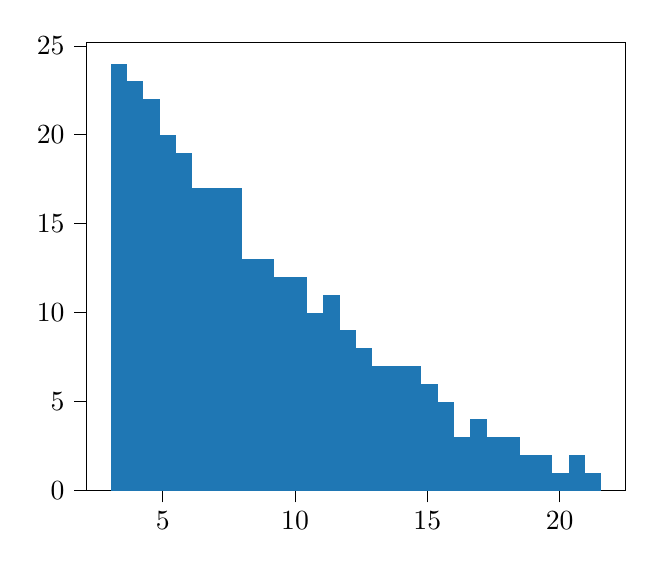
\begin{tikzpicture}

\definecolor{darkgray176}{RGB}{176,176,176}
\definecolor{steelblue31119180}{RGB}{31,119,180}

\begin{axis}[
tick align=outside,
tick pos=left,
x grid style={darkgray176},
xmin=2.10505, xmax=22.50125,
xtick style={color=black},
y grid style={darkgray176},
ymin=0, ymax=25.2,
ytick style={color=black}
]
\draw[draw=none,fill=steelblue31119180] (axis cs:3.03215,0) rectangle (axis cs:3.65021666666667,24);
\draw[draw=none,fill=steelblue31119180] (axis cs:3.65021666666667,0) rectangle (axis cs:4.26828333333333,23);
\draw[draw=none,fill=steelblue31119180] (axis cs:4.26828333333333,0) rectangle (axis cs:4.88635,22);
\draw[draw=none,fill=steelblue31119180] (axis cs:4.88635,0) rectangle (axis cs:5.50441666666667,20);
\draw[draw=none,fill=steelblue31119180] (axis cs:5.50441666666667,0) rectangle (axis cs:6.12248333333333,19);
\draw[draw=none,fill=steelblue31119180] (axis cs:6.12248333333333,0) rectangle (axis cs:6.74055,17);
\draw[draw=none,fill=steelblue31119180] (axis cs:6.74055,0) rectangle (axis cs:7.35861666666667,17);
\draw[draw=none,fill=steelblue31119180] (axis cs:7.35861666666667,0) rectangle (axis cs:7.97668333333333,17);
\draw[draw=none,fill=steelblue31119180] (axis cs:7.97668333333333,0) rectangle (axis cs:8.59475,13);
\draw[draw=none,fill=steelblue31119180] (axis cs:8.59475,0) rectangle (axis cs:9.21281666666667,13);
\draw[draw=none,fill=steelblue31119180] (axis cs:9.21281666666667,0) rectangle (axis cs:9.83088333333333,12);
\draw[draw=none,fill=steelblue31119180] (axis cs:9.83088333333333,0) rectangle (axis cs:10.44895,12);
\draw[draw=none,fill=steelblue31119180] (axis cs:10.44895,0) rectangle (axis cs:11.0670166666667,10);
\draw[draw=none,fill=steelblue31119180] (axis cs:11.0670166666667,0) rectangle (axis cs:11.6850833333333,11);
\draw[draw=none,fill=steelblue31119180] (axis cs:11.6850833333333,0) rectangle (axis cs:12.30315,9);
\draw[draw=none,fill=steelblue31119180] (axis cs:12.30315,0) rectangle (axis cs:12.9212166666667,8);
\draw[draw=none,fill=steelblue31119180] (axis cs:12.9212166666667,0) rectangle (axis cs:13.5392833333333,7);
\draw[draw=none,fill=steelblue31119180] (axis cs:13.5392833333333,0) rectangle (axis cs:14.15735,7);
\draw[draw=none,fill=steelblue31119180] (axis cs:14.15735,0) rectangle (axis cs:14.7754166666667,7);
\draw[draw=none,fill=steelblue31119180] (axis cs:14.7754166666667,0) rectangle (axis cs:15.3934833333333,6);
\draw[draw=none,fill=steelblue31119180] (axis cs:15.3934833333333,0) rectangle (axis cs:16.01155,5);
\draw[draw=none,fill=steelblue31119180] (axis cs:16.01155,0) rectangle (axis cs:16.6296166666667,3);
\draw[draw=none,fill=steelblue31119180] (axis cs:16.6296166666667,0) rectangle (axis cs:17.2476833333333,4);
\draw[draw=none,fill=steelblue31119180] (axis cs:17.2476833333333,0) rectangle (axis cs:17.86575,3);
\draw[draw=none,fill=steelblue31119180] (axis cs:17.86575,0) rectangle (axis cs:18.4838166666667,3);
\draw[draw=none,fill=steelblue31119180] (axis cs:18.4838166666667,0) rectangle (axis cs:19.1018833333333,2);
\draw[draw=none,fill=steelblue31119180] (axis cs:19.1018833333333,0) rectangle (axis cs:19.71995,2);
\draw[draw=none,fill=steelblue31119180] (axis cs:19.71995,0) rectangle (axis cs:20.3380166666667,1);
\draw[draw=none,fill=steelblue31119180] (axis cs:20.3380166666667,0) rectangle (axis cs:20.9560833333333,2);
\draw[draw=none,fill=steelblue31119180] (axis cs:20.9560833333333,0) rectangle (axis cs:21.57415,1);
\end{axis}

\end{tikzpicture}
